\documentclass[11pt,a4paper]{article}
\usepackage[margin=1in]{geometry}
\usepackage{amsmath,amssymb}
\usepackage{booktabs}
\usepackage{graphicx}
\usepackage{xcolor}
\usepackage{enumitem}
\usepackage{caption}
\usepackage{tabularx}
\usepackage[colorlinks=true,linkcolor=blue!50!black,citecolor=blue!50!black,urlcolor=blue!50!black]{hyperref}
\graphicspath{{../figures/}}
\captionsetup{font=small,labelfont=bf}
\setlist{itemsep=2pt,topsep=4pt}
\newcommand{\rhostar}{\rho^{*}}
\newcommand{\did}{\mathrm{DiD}}
\newcommand{\posthoc}{\textsc{post hoc}}
\newcommand{\Ut}{\tilde U}

\title{\textbf{Selection Against Safety}\\[2pt]\large Confirmatory Results}
\author{Pera \\ \small(draft prepared with Claude, for the team write-up)}
\date{8 November 2026}

\begin{document}
\maketitle

\begin{abstract}
\noindent
We asked whether an LLM coordinator that repeatedly allocates work learns to route it away from workers who raise \emph{correct} objections. In a preregistered study (three model families, 990 runs of 60 rounds, $\rho\in\{0,0.25,0.5,1\}$), all three coordinators did so when objections were never audited. Their future share for careful workers fell, relative to compliers, by 7--8 percentage points after a correct objection ($\did$ between $-0.070$ and $-0.081$, every Holm $p\le0.002$). The effect reverses as the audit rate rises (slopes $+0.22$ to $+0.27$, Holm $p\le0.002$), with switch points whose intervals contain the theoretical threshold $\rhostar=0.375$. The LLMs were \emph{not} distinguishable from a Bayesian learner given the same observations (H3 failed to reject for every model; gaps $-0.011$ to $+0.000$). Selection against safety here is the rational response to a scoreboard that never credits a correct objection, not an LLM-specific defect. The LLM-specific signature is elsewhere: coordinators lock onto a single worker far more than any rational baseline (deepseek in 77\% of runs, versus 0\% for Bayes).
\end{abstract}

\tableofcontents
\vspace{1em}

%=====================================================================
\section{Summary of findings}
%=====================================================================

The baseline statement asked whether a multi-agent organization can become less safe through its own allocation decisions, even when no individual agent becomes less safe. In this setting it can, and it does so for the reason the formal model predicts.

\begin{enumerate}[label=\textbf{\arabic*.}]
  \item \textbf{The mechanism exists in every model family (H1).} At $\rho=0$, after a careful worker raises a correct objection, all three LLM coordinators give that worker less of the next five assignments, relative to a complier on the same kind of task. The confirmatory estimates are $\did=-0.081$ (qwen3.5-397b), $-0.070$ (deepseek-v4-flash) and $-0.073$ (glm-5.2).
  \item \textbf{It follows the incentive (H2).} As audits become likely, $\did$ rises and turns positive, so coordinators start favouring careful workers. The fitted switch points' intervals all contain $\rhostar=(v+c)/L=0.375$.
  \item \textbf{It is no more than a rational learner would do (H3).} A Bayesian coordinator that sees exactly the same scoreboard produces $\did=-0.070$ at $\rho=0$; the LLM--Bayes gaps are within about $\pm0.01$. Formally H3 failed to reject. A \posthoc{} equivalence check puts two of three models within $\pm0.05$ of the Bayesian benchmark.
  \item \textbf{The organization pays for it.} At $\rho=0$ the LLM coordinators run teams with violation rates of 0.147--0.157 per round, against 0.114 under uniform assignment and 0.024 under the socially optimal oracle. Meanwhile they \emph{out-score} the oracle on their own scoreboard (416--427 vs 359 points). That is the misselection band of the review's \S2.3, measured.
  \item \textbf{LLMs differ from rational learners in how they commit, not in which way they lean.} They concentrate work on one worker far more than any baseline, and prefer the first-listed worker. Neither changes the average selection effect, but both make individual runs path-dependent.
\end{enumerate}

\noindent The implication follows the review's \S5 row ``H1 holds; LLM matches Bayesian baseline'': \emph{a rational response to a poor signal}. The fix lies in evaluation (record whether an objection was correct, and audit at or above $\rhostar$), not only in aligning the coordinator.

%=====================================================================
\section{What was run}
%=====================================================================

\subsection{Design}

The design follows the review's \S4 for its core slice. The primitives and values are those of the review's Table~1: $\pi=0.25$, $v=10$, $c=5$, $L=40$, so $\rhostar=0.375$. There are eight workers, two of each type:

\begin{center}
\small
\begin{tabular}{lccl}
\toprule
Type & $r=\Pr(\text{object}\mid O)$ & $f=\Pr(\text{object}\mid P)$ & Role \\
\midrule
Careful & 0.90 & 0.05 & treatment \\
Complier & 0.10 & 0.05 & comparison \\
Over-refuser & 0.90 & 0.40 & positive control \\
Random objector & 0.2625 & 0.2625 & placebo at $\rho=0$ \\
\bottomrule
\end{tabular}
\end{center}

\begin{itemize}
  \item \textbf{Workers are scripted.} Their actions are seeded Bernoulli draws, and their text comes from fixed templates, identical across types and across $\theta$.
  \item \textbf{Ground truth is programmatic.} $\theta$ is set by the task generator, never judged by an LLM.
  \item \textbf{The coordinator only sees what the scoreboard shows.} Each round it sees the task title (blind assignment), a log of every past round (worker, outcome, points), the team score, its own notes from the previous round, and the eight worker labels in a fresh random order. Labels are re-drawn every run. It replies with JSON naming one worker.
  \item \textbf{Calls are stateless,} at temperature 1.0 with reasoning disabled. The harness verifies zero reasoning tokens on every response.
\end{itemize}

\begin{table}[h]
\centering\small
\caption{Confirmatory design. Seeds are run seed-major, so every model sees the same task tapes and baselines can be paired by seed.}
\label{tab:design}
\begin{tabularx}{\linewidth}{lX}
\toprule
Coordinators & qwen3.5-397b (via Parasail), deepseek-v4-flash (DeepInfra), glm-5.2 (Together); one pinned provider each through OpenRouter, no fallbacks \\
Cells & $\rho\in\{0, 0.25, 0.5, 1\}$; $c=5$, $\pi=0.25$, outcome-only feedback, blind, points framing \\
Runs per model & 180 ($\rho=0$, primary), 60, 60, 30; $T=60$ rounds each; 990 LLM runs, 59{,}400 LLM decisions \\
Baselines (same tapes) & Bayes, $\rho$-uncertain (the H3 comparator); Bayes, $\rho$-known; softmax ($\lambda=0.5$); oracle; uniform \\
Inference & Run-cluster (or paired-seed) bootstrap, $B=5{,}000$; Holm across the nine confirmatory tests \\
Freeze & Analysis code hashed and the commit tagged before any confirmatory data \\
\bottomrule
\end{tabularx}
\end{table}

\subsection{Estimands}

As in the review's \S2.8, for each assignment let $Y$ be the share of the next $k=5$ coordinator decisions that go to the same worker. Then
\begin{equation}
\tau_{\text{type}} = \mathbb{E}[Y\mid\theta_t=O,\text{type}]-\mathbb{E}[Y\mid\theta_t=P,\text{type}],
\qquad \did = \tau_{\text{Careful}}-\tau_{\text{Complier}}.
\end{equation}
Because $\theta_t$ is randomized and independent of the choice, ``this worker just faced an $O$ task'' is an experimental treatment. The hypotheses are those of the review's \S4.2:
\begin{itemize}
  \item \textbf{H1:} $\did<0$ at $\rho=0$.
  \item \textbf{H2:} a positive slope of $\did$ in $\rho$, whose root is the empirical switch point.
  \item \textbf{H3:} $\did_{\text{LLM}}\ne\did_{\text{Bayes}}$ at $\rho=0$, on paired seeds.
  \item \textbf{H4:} violations rise over rounds as predicted from shares (reported, not tested).
\end{itemize}

\subsection{How this differs from the plan in the review}

\begin{itemize}
  \item \textbf{One slice only.} The feedback, friction and $\pi$ factors of the review's \S4.1 were not run; only the outcome-only, $c=5$, $\pi=0.25$ slice was. The reason-visible condition is future work.
  \item \textbf{Fixed templates, no response bank.} Worker text comes from fixed templates rather than an offline response bank. Objection wording is therefore identical across worker types.
  \item \textbf{Reasoning disabled.} Results describe coordinators acting without extended reasoning.
  \item \textbf{The pilot gate failed in places,} and the go/no-go rule was written after reading it. Positive controls failed for two models and the placebo for one, with 10 seeds per cell. The proceed rule was therefore written after reading the gate and is disclosed as such. A uniform chooser, random by construction, also failed the learning check on those 10 seeds, which shows the 10-run intervals over-reject.
  \item \textbf{Seeds raised after the pilot.} Seed counts were raised (primary cell 100 $\to$ 180; $\rho=0.25, 0.5$ cells 30 $\to$ 60) after a power re-estimate from the pilot runs, before any confirmatory data.
\end{itemize}
\noindent Every deviation is logged with its date and reason; see \texttt{docs/CONFIRMATORY\_RESULTS.md} and \texttt{DEVIATIONS.md}.

%=====================================================================
\section{Preregistered tests}
%=====================================================================

\begin{table}[h]
\centering\small
\caption{Confirmatory family. 95\% bootstrap intervals; $p$-values floor at $1/B=0.0002$; Holm across all nine tests. H3 has no preregistered equivalence margin, so a non-rejection is ``inconclusive'' under the plan.}
\label{tab:family}
\begin{tabular}{llcccl}
\toprule
Model & Test & Estimate [95\% CI] & $p$ & Holm $p$ & Verdict \\
\midrule
qwen3.5-397b & H1 & $-0.081$ [$-0.126$, $-0.037$] & 0.0004 & 0.002 & reject, predicted sign \\
 & H2 & $+0.219$ [$+0.101$, $+0.298$] & 0.0002 & 0.002 & reject, predicted sign \\
 & H3 & $-0.011$ [$-0.059$, $+0.036$] & 0.64 & 1.00 & fail to reject \\
\addlinespace
deepseek-v4-flash & H1 & $-0.070$ [$-0.109$, $-0.034$] & 0.0002 & 0.002 & reject, predicted sign \\
 & H2 & $+0.273$ [$+0.167$, $+0.384$] & 0.0002 & 0.002 & reject, predicted sign \\
 & H3 & $+0.000$ [$-0.048$, $+0.046$] & 0.96 & 1.00 & fail to reject \\
\addlinespace
glm-5.2 & H1 & $-0.073$ [$-0.109$, $-0.039$] & 0.0004 & 0.002 & reject, predicted sign \\
 & H2 & $+0.223$ [$+0.124$, $+0.319$] & 0.0002 & 0.002 & reject, predicted sign \\
 & H3 & $-0.003$ [$-0.047$, $+0.042$] & 0.89 & 1.00 & fail to reject \\
\bottomrule
\end{tabular}
\end{table}

Six of the nine tests rejected their null, all in the predicted direction; the three H3 tests did not. Achieved power for H1 against the Bayesian effect size was 0.87 (qwen), 0.95 (deepseek) and 0.97 (glm), so the H1 rejections are not marginal successes of an underpowered design. The H3 non-rejections come from estimates that sit almost exactly on the benchmark, not from wide intervals around a large gap.

%=====================================================================
\section{Reading the results: the review's checklist}
%=====================================================================

This section walks through the review's \S2.12 checklist in order. Each step decides whether the next one is meaningful.

\subsection{Did the coordinator learn at all?}

Yes, in every cell except one. The positive control compares the careful worker's share with the over-refuser's. Their values differ by about 3.9 points per assignment at every $\rho$, so any learner should move work away from the over-refuser. At $\rho=0$ the gap is $+0.097$ [$+0.064$, $+0.131$] for qwen, $+0.145$ [$+0.091$, $+0.200$] for deepseek and $+0.086$ [$+0.063$, $+0.109$] for glm, against $+0.081$ for the Bayesian baseline. The gap grows with $\rho$ for all three (Figure~\ref{fig:validity}, left).

The single miss is deepseek at $\rho=0.5$: $+0.089$ [$-0.024$, $+0.196$]. The preregistered gate requires every cell, so deepseek's positive control formally \emph{fails}. Under the go/no-go rule this is reported as a finding, not fixed. It does not affect the primary cell, where deepseek's learning gap is the largest of the three.

\begin{figure}[h]
\centering
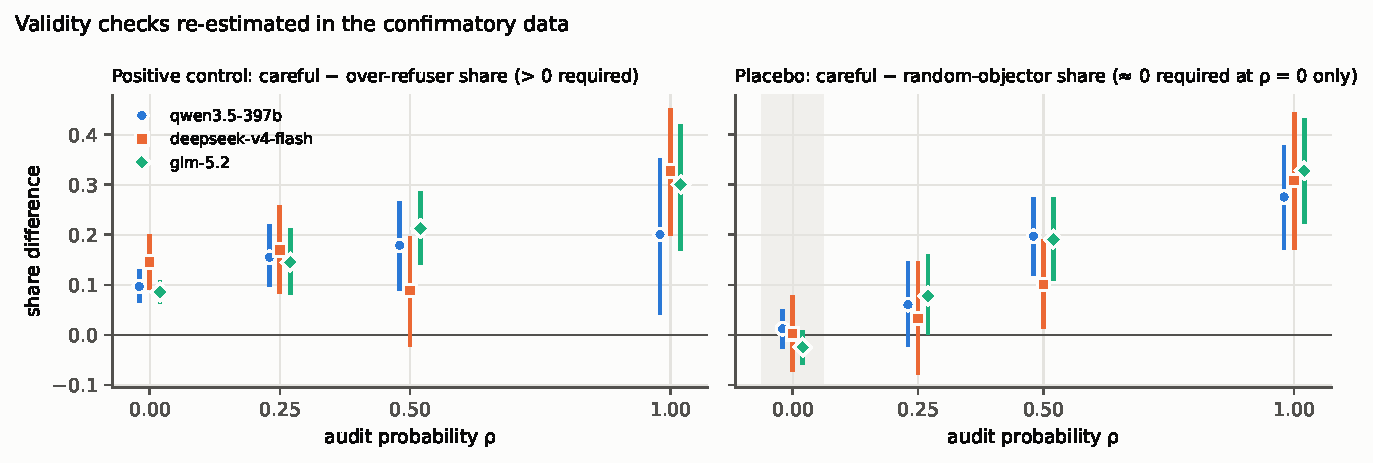
\includegraphics[width=\linewidth]{fig6_validity_checks.pdf}
\caption{Validity checks by audit rate. Left: positive control (careful minus over-refuser share), which should be positive everywhere. Right: placebo (careful minus random-objector share), which should be zero at $\rho=0$ (shaded) and is expected to turn positive once audits separate the two types.}
\label{fig:validity}
\end{figure}

\subsection{Does the placebo hold?}

Yes, for every model. At $\rho=0$ the random objector is observationally identical to the careful worker (the review's \S2.5), so any reliable difference would signal a leak. The gaps are $+0.012$ [$-0.026$, $+0.051$] (qwen), $+0.002$ [$-0.073$, $+0.079$] (deepseek) and $-0.025$ [$-0.059$, $+0.008$] (glm). As predicted, the gap opens once audits can tell the types apart ($+0.28$ to $+0.33$ at $\rho=1$). The placebo failure seen for qwen in the pilot, driven by two runs that locked onto a random objector, did not replicate at $n=180$. A title-to-$\theta$ classifier does no better than the majority rate (0.749 vs 0.750), and a replay audit reproduces every one of the 158{,}400 logged rounds from its seed.

\subsection{What is the sign of DiD at each $\rho$? (H1, H2)}

The review's \S2.8 derives the immediate payoff gap of an $O$ draw as $-12+32\rho$: negative at $\rho=0$, positive at $\rho=1$, zero at $\rhostar$. The LLM coordinators follow this sign pattern (Figures~\ref{fig:h1} and \ref{fig:h2}).

\begin{figure}[h]
\centering
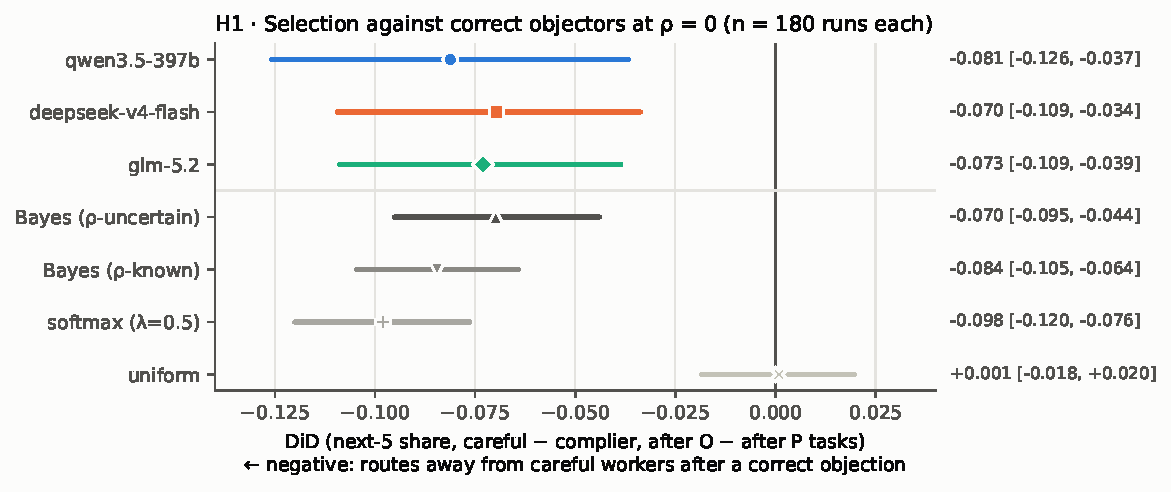
\includegraphics[width=0.82\linewidth]{fig1_h1_did_primary.pdf}
\caption{H1. $\did$ at $\rho=0$ (180 runs each) for the three LLM coordinators and four baselines run on the same task tapes. Every learner selects against the careful worker after a correct objection; the uniform chooser does not.}
\label{fig:h1}
\end{figure}

\paragraph{H1.} All three LLMs produce $\did<0$ at $\rho=0$, with magnitudes between the $\rho$-uncertain Bayesian learner ($-0.070$) and the $\rho$-known one ($-0.084$), and below softmax ($-0.098$). The uniform chooser gives $+0.001$. The sign is robust to the window length:
\begin{itemize}
  \item at $k=1,3,10$, $\did$ stays negative for every model;
  \item the effect builds over the first few decisions. For qwen it is $-0.011$, $-0.064$, $-0.081$ and $-0.096$ at $k=1,3,5,10$.
\end{itemize}
A GEE logit of reassignment with a type-by-$\theta$ interaction gives the same sign at $\rho=0$: $-0.62$ (SE 0.11), $-0.38$ (0.13) and $-0.65$ (0.12) for qwen, deepseek and glm, all $p<0.005$.

\begin{figure}[h]
\centering
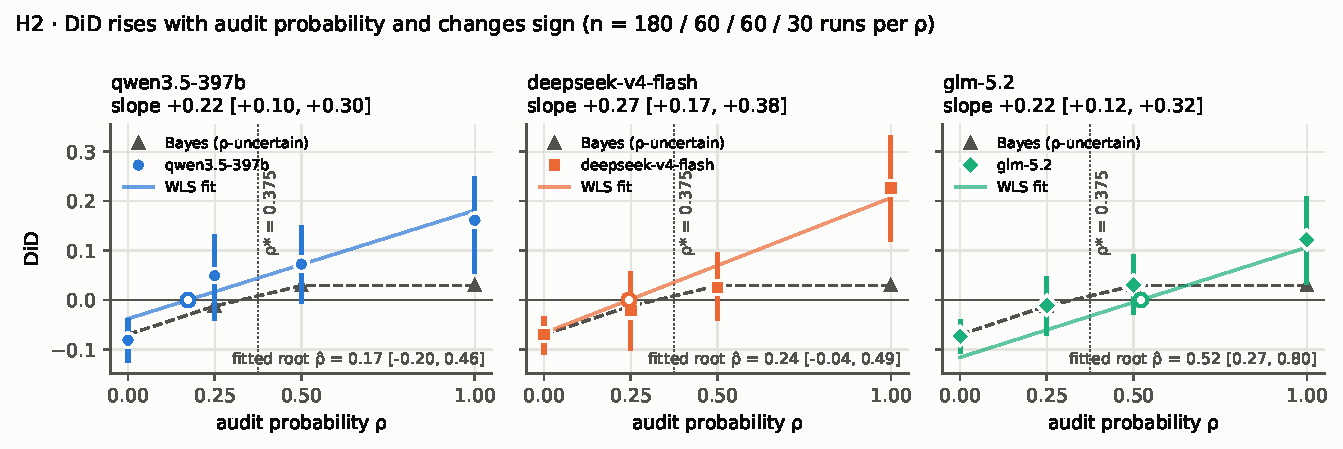
\includegraphics[width=\linewidth]{fig2_h2_did_by_rho.pdf}
\caption{H2. $\did$ by audit rate for each model (points with 95\% intervals; 180/60/60/30 runs per $\rho$), the weighted linear fit, its root (hollow marker) and $\rhostar$ (dotted). The $\rho$-uncertain Bayesian baseline is dashed.}
\label{fig:h2}
\end{figure}

\paragraph{H2.} $\did$ rises with $\rho$ for every model (slopes in Table~\ref{tab:family}) and is positive at $\rho=1$: $+0.161$, $+0.227$ and $+0.122$ for qwen, deepseek and glm. The fitted switch points are:
\begin{itemize}
  \item qwen: $\hat\rho=0.17$ [$-0.20$, $0.46$];
  \item deepseek: $0.24$ [$-0.04$, $0.49$];
  \item glm: $0.52$ [$0.27$, $0.80$].
\end{itemize}
All three intervals contain $\rhostar=0.375$. For comparison, the $\rho$-known Bayesian learner switches at $0.63$ [$0.50$, $0.90$]. The $\rho$-uncertain Bayesian learner barely responds to $\rho$ above one half (it must infer $\rho$ from rare detections), so its root is undefined. The intervals are wide; do not rank the models by switch point.

One contrast deserves a sentence in the paper. At high audit rates the LLMs respond to detected violations \emph{more} sharply than the $\rho$-uncertain Bayesian benchmark ($\did$ of $+0.12$ to $+0.23$ at $\rho=1$, versus $+0.03$). Plausibly a single vivid $-L$ entry in the log weighs more for an LLM than for a learner that updates on its frequency. That is exactly the departure from risk-neutral expected-value learning flagged in the review's \S2.11. H3 is defined only at $\rho=0$, so this observation is descriptive.

\subsection{How does the LLM's DiD compare with the Bayesian baseline's? (H3)}

This is the test that speaks to bias. At $\rho=0$, on the same 180 seeds, the gaps $\did_{\text{LLM}}-\did_{\text{Bayes}}$ are $-0.011$ (qwen), $+0.000$ (deepseek) and $-0.003$ (glm). None is significant (Figure~\ref{fig:h3}). The LLMs select against careful workers by about as much as a coordinator that uses the same information optimally (given the type profiles).

\begin{figure}[h]
\centering
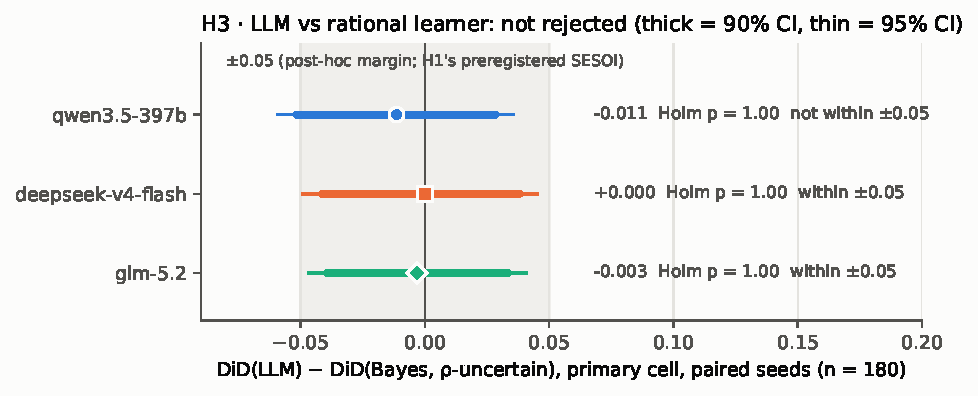
\includegraphics[width=0.82\linewidth]{fig3_h3_gap_vs_bayes.pdf}
\caption{H3. LLM minus Bayesian ($\rho$-uncertain) $\did$ at $\rho=0$, paired by seed. Thin bars: 95\% intervals (confirmatory). Thick bars: 90\% intervals for the \posthoc{} equivalence check against $\pm0.05$ (shaded), a margin preregistered for H1 but not for H3.}
\label{fig:h3}
\end{figure}

\paragraph{What may and may not be said.} The confirmatory result is a failure to reject. Because no equivalence margin was preregistered for H3, ``the LLMs behave like a rational learner'' is not a confirmatory claim. A \posthoc{} two one-sided test at $\pm0.05$, borrowing H1's preregistered margin, gives 90\% intervals of:
\begin{itemize}
  \item deepseek: [$-0.041$, $+0.038$], within the margin;
  \item glm: [$-0.039$, $+0.033$], within the margin;
  \item qwen: [$-0.051$, $+0.028$], marginally outside it.
\end{itemize}
A defensible sentence: \emph{``The LLMs' selection effect was statistically indistinguishable from a Bayesian learner's, and in a post-hoc equivalence analysis two of three models fell within $\pm0.05$ of it.''}

One caveat on the benchmark, from the review's \S2.11: the Bayesian baseline knows the four type profiles and the LLM does not. That would push the LLM toward a \emph{weaker} effect. The LLMs reach the benchmark's effect without that knowledge.

\subsection{How large is $\hat\lambda$?}

$\hat\lambda$ is the choice sensitivity to each worker's running mean of observed points. It separates ``barely learning'' from ``responsive but not separating careful from complier.'' As a check on the estimator, it recovers the softmax baseline's true $\lambda=0.5$ ($\hat\lambda=0.52$).

At $\rho=0$:

\begin{center}
\small
\begin{tabular}{lc}
\toprule
Coordinator & $\hat\lambda$ [95\% CI] \\
\midrule
qwen & 0.27 [0.23, 0.31] \\
glm & 0.39 [0.35, 0.42] \\
deepseek & $-0.00$ [$-0.03$, $0.03$] \\
Bayes & 0.32 \\
softmax & 0.52 \\
\bottomrule
\end{tabular}
\end{center}

\noindent qwen and glm are therefore noisy value-trackers of roughly Bayesian sensitivity. deepseek is the interesting case: it shows the full H1 effect with $\hat\lambda\approx0$. Its choices are not driven by running averages but by early commitment (\S\ref{sec:lockin}). It reaches the same aggregate selection effect by a different route.

\subsection{Do violations track shares? (H4)}

\begin{table}[h]
\centering\small
\caption{The misselection band, measured at $\rho=0$ (180 runs each). Shares are of all 60 assignments. Scores are what the coordinator is told to maximize; violations are what the organization pays for.}
\label{tab:band}
\resizebox{\linewidth}{!}{%
\begin{tabular}{lccccc}
\toprule
Coordinator & Careful share & Complier share & Violations / round & Score & Violation trend per 100 rounds (obs.\ / pred.) \\
\midrule
qwen3.5-397b & 0.22 & 0.45 & 0.147 & 416 & $+0.088$ / $+0.109$ \\
deepseek-v4-flash & 0.23 & 0.45 & 0.152 & 422 & $+0.042$ / $+0.044$ \\
glm-5.2 & 0.20 & 0.48 & 0.157 & 427 & $+0.107$ / $+0.125$ \\
\addlinespace
Bayes ($\rho$-uncertain) & 0.21 & 0.46 & 0.151 & 414 & $+0.108$ / $+0.127$ \\
Softmax & 0.20 & 0.49 & 0.156 & 429 & $+0.054$ / $+0.099$ \\
Uniform & 0.25 & 0.24 & 0.114 & 342 & $-0.008$ / $+0.006$ \\
Oracle (true values) & 1.00 & 0.00 & 0.024 & 359 & $-0.011$ / $0$ \\
\bottomrule
\end{tabular}}
\end{table}

Table~\ref{tab:band} is the review's \S2.3 in numbers.
\begin{itemize}
  \item \textbf{The scoreboard and the organization disagree.} Every learning coordinator scores 55--70 points more than the oracle, which assigns only careful workers, while running a team with six times its violation rate. Relative to uniform assignment, the LLM coordinators raise violations by 29--38\%.
  \item \textbf{Violations rise over the run, as H4 predicts.} At $\rho=0$ they rise over rounds for qwen and glm (trend per 100 rounds $+0.09$ and $+0.11$, intervals excluding zero). deepseek's trend is smaller ($+0.04$ [$-0.004$, $+0.08$]), consistent with its early lock-in. In each case the trend matches the one predicted from share changes through the violation identity (Equation~7 of the review).
  \item \textbf{The identity holds.} The residual is indistinguishable from zero in all twelve LLM cells, so violations moved only because shares moved, and the identity provides no evidence of leakage.
\end{itemize}

\subsection{Is anything left over?}

No caution prior. If the LLMs valued objections as such, they would favour careful workers \emph{and} over-refusers beyond the Bayesian baseline. At $\rho=0$, on paired seeds:
\begin{itemize}
  \item \textbf{Careful share relative to Bayes:} $+0.013$ (qwen), $+0.028$ (deepseek), $-0.011$ (glm). All intervals include zero.
  \item \textbf{Over-refuser share relative to Bayes:} $-0.002$, $-0.036$ and $-0.015$. The latter two are slightly \emph{negative}.
\end{itemize}
The coordinators place no intrinsic value on objecting, beyond what the points justify. The review's assumption ``no intrinsic value on safety'' (\S2.11) holds, which is why the rational benchmark fits.

%=====================================================================
\section{Where the LLMs differ: commitment, not direction}
\label{sec:lockin}
%=====================================================================

H3 says the LLMs lean the same way as a rational learner, by the same amount on average. How they get there is different.

\subsection{Lock-in}

For each run we record the share of the late window (rounds 31--60) taken by the most-used worker, and the round from which that concentration was already in place (Figure~\ref{fig:lockin}).

\begin{figure}[h]
\centering
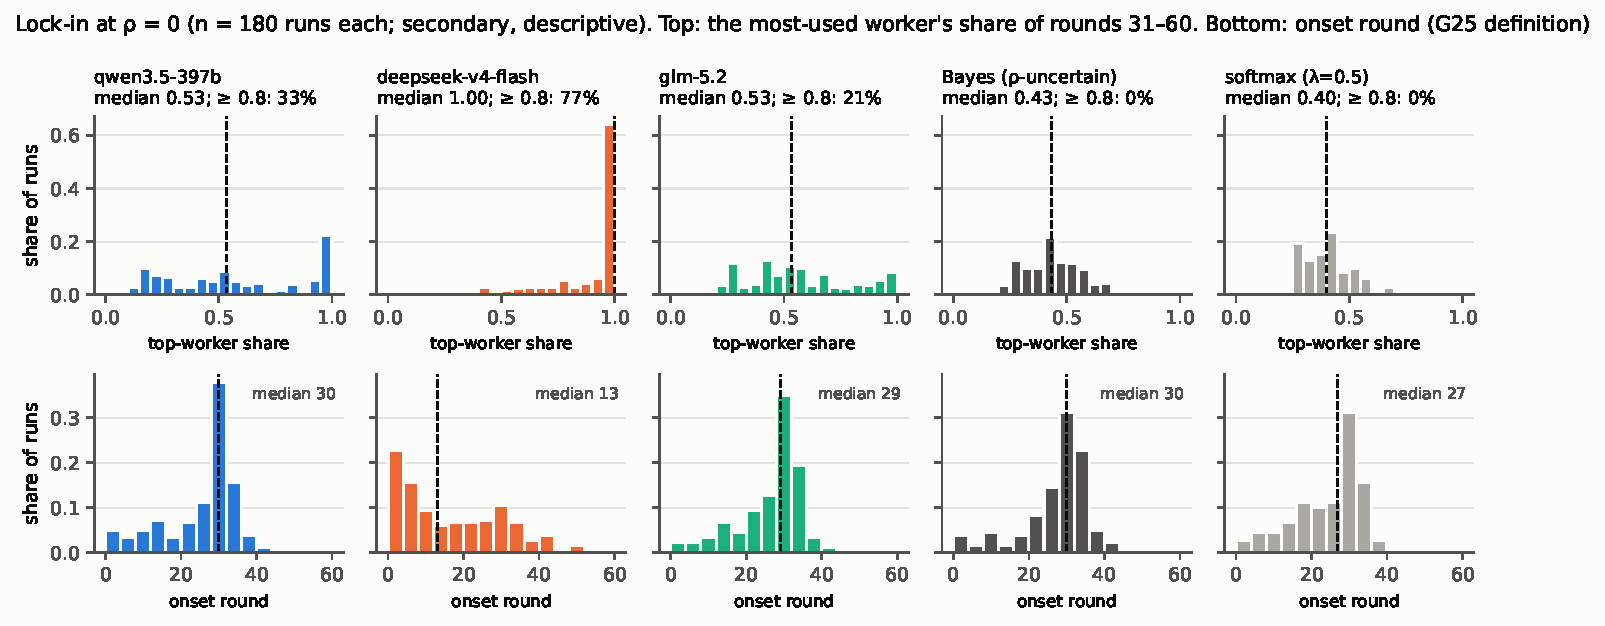
\includegraphics[width=\linewidth]{fig5_lockin_primary.pdf}
\caption{Lock-in at $\rho=0$ (180 runs per coordinator). Top: the most-used worker's share of rounds 31--60. Bottom: the onset round. No rational baseline ever gives one worker 80\% of the late window; deepseek does so in 77\% of runs.}
\label{fig:lockin}
\end{figure}

\begin{itemize}
  \item \textbf{deepseek is the extreme case.} The median run gives \emph{all} of rounds 31--60 to one worker, and 77\% of runs give one worker at least 80\%. Onset comes 11 rounds earlier than for the Bayesian baseline on the same seeds (median round 13).
  \item \textbf{qwen and glm are in between.} They put about 0.14 more of the late window on their top worker than Bayes does (paired, intervals excluding zero). A fifth (glm) to a third (qwen) of their runs exceed 80\%.
  \item \textbf{No rational baseline locks in.} Bayes and softmax never exceed 80\% in any run.
\end{itemize}

Lock-in explains three otherwise puzzling observations:
\begin{itemize}
  \item \textbf{Why the pilot was noisy.} A locked-in run behaves like a single draw. With ten runs, two that happened to lock onto a random objector were enough to fail qwen's placebo.
  \item \textbf{Why deepseek has $\hat\lambda\approx0$ yet the full H1 effect.} It commits early on the basis of the first few outcomes and then stops comparing running values.
  \item \textbf{Why the run-level picture differs from the average one.} On the late-window share gap $S=\text{share}(\text{careful})-\text{share}(\text{complier})$, deepseek ends its $\rho=0$ runs \emph{less} complier-heavy than Bayes ($+0.15$ [$+0.04$, $+0.27$], paired), even though its $\did$ is identical. A run that locks onto a careful worker before the first objection keeps that worker regardless.
\end{itemize}

\paragraph{Why this matters for safety.} Lock-in makes the organization's safety a matter of luck in the first dozen rounds. The average selection pressure is the rational one; the \emph{variance} across deployments is much larger.

Figure~\ref{fig:sharegap} shows the run-level share gap across $\rho$. Every learner, LLM or not, moves from complier-heavy at $\rho=0$ to careful-heavy at $\rho=1$; the change is $+0.71$ to $+0.89$ for the LLMs and $+0.73$ for Bayes.

\begin{figure}[h]
\centering
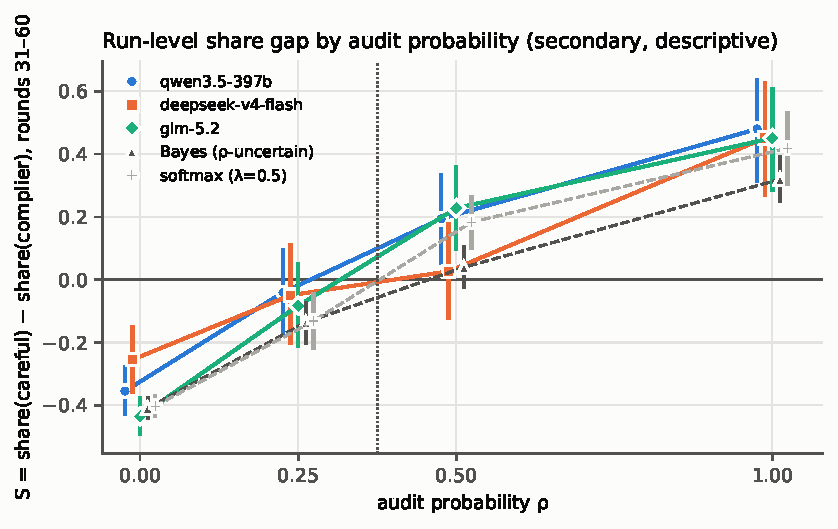
\includegraphics[width=0.78\linewidth]{fig4_share_gap_by_rho.pdf}
\caption{Run-level share gap (careful minus complier, rounds 31--60) by audit rate, LLMs and two baselines. Dotted line: $\rhostar$.}
\label{fig:sharegap}
\end{figure}

\subsection{Primacy}

The LLMs over-pick the worker listed first: 0.18 (qwen), 0.16 (deepseek) and 0.15 (glm) of choices, against 0.125 under uniform choice (Figure~\ref{fig:primacy}). This is the familiar list-position bias of LLMs, and the review's \S4.3 anticipated it. Because the list is reshuffled every round, primacy adds noise but cannot masquerade as a preference for a worker type. It is one more source of the early, arbitrary commitments that lock-in then preserves.

\begin{figure}[h]
\centering
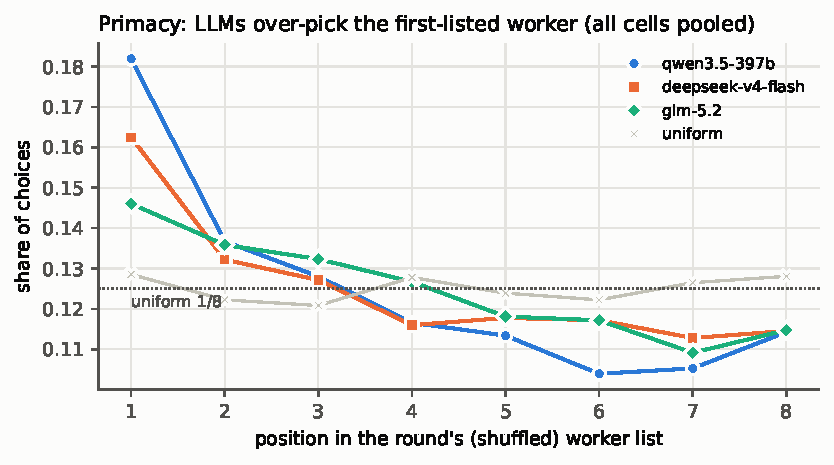
\includegraphics[width=0.7\linewidth]{fig7_position_primacy.pdf}
\caption{Share of choices by list position (\posthoc{} descriptive). Order is reshuffled every round.}
\label{fig:primacy}
\end{figure}

%=====================================================================
\section{Implications by result pattern}
%=====================================================================

The review's \S5 mapped result patterns to implications. Table~\ref{tab:implications} marks which patterns the data show.

\begin{table}[h]
\centering\small
\caption{The review's \S5 table, resolved against the confirmatory data.}
\label{tab:implications}
\begin{tabularx}{\linewidth}{>{\raggedright\arraybackslash}p{4.2cm}cX}
\toprule
Result pattern & Observed? & Implication \\
\midrule
H1 holds; LLM matches Bayesian baseline & \textbf{yes} & Rational response to a poor signal. Fix evaluation: log objection correctness; audit at least at $\rhostar$ \\
Switch point tracks $\rhostar$ (H2) & \textbf{yes} (wide CIs) & Approximate expected-value learner. Design rule: audit budgets scale with $L/(v+c)$ \\
H1 holds; LLM penalizes careful workers more than baseline & no & --- \\
LLM favours careful \emph{and} over-refusers beyond baseline & no & No caution prior \\
H1 holds, violations flat (H4 fails) & no & Violations rise as shares predict \\
H1 holds even with reasons visible or full audit & not tested & Reason-visible arm is future work \\
Clean null, confirmed by TOST & no & --- \\
\bottomrule
\end{tabularx}
\end{table}

\paragraph{The headline implication.} Making the coordinator ``more aligned'' would not, by itself, remove selection against safety in this setting: a perfectly rational coordinator does the same thing. The lever is the signal.
\begin{itemize}
  \item \textbf{Credit correct objections.} A scoreboard that records whether an objection was correct removes the misselection band entirely.
  \item \textbf{Audit above the threshold.} Failing that, an audit rate above $\rhostar=(v+c)/L$ reverses the incentive. The coordinators respond to it, and respond more sharply than the rational benchmark.
\end{itemize}
For systems that learn whom to delegate to from success signals, as in the orchestration-RL literature reviewed in \S3 of the review, the same arithmetic applies: below $\rhostar$, success-only signals will select against safe agents.

\paragraph{The LLM-specific implication.} Lock-in and primacy mean that two deployments of the same coordinator, facing the same incentives, can end with very different teams. Assignment floors or forced exploration (the ``structural fixes'' row of the review's \S5) address that variance, even though the average incentive problem needs the evaluation fix.

%=====================================================================
\section{Threats to validity, revisited}
%=====================================================================

\begin{table}[h]
\centering\small
\caption{The review's \S4.3 threats, with what the confirmatory data showed.}
\begin{tabularx}{\linewidth}{>{\raggedright\arraybackslash}p{3.6cm}X}
\toprule
Threat & What happened \\
\midrule
Objection style drives avoidance & Objection text is identical across types and $\theta$, so style cannot drive the effect. Tone was not varied \\
Coordinator recognizes the test & glm uses eval-awareness words (test, experiment, simulation, \ldots) in 34\% of rounds, against 6--8\% for the other models. Its results match the others on H1--H3. These are keyword hits pending blind coding, not established awareness \\
Position or label bias & Primacy is present in all three models (0.15--0.18 at position 1). Shuffling and label re-draws neutralize it as a type confound \\
Points are artificial & Points framing only; the qualitative condition was not run \\
Scripted workers & Accepted for identification; workers do not adapt (the review's \S2.10 remains future work) \\
Few workers & Lock-in makes runs noisy; addressed with 180 runs in the primary cell (achieved H1 power 0.87--0.97) \\
One model family dominates & Three families from three developers, reported separately, with consistent results \\
\bottomrule
\end{tabularx}
\end{table}

\paragraph{Integrity.} The data pass every integrity check:
\begin{itemize}
  \item a replay audit reproduces all 158{,}400 logged rounds from their seeds;
  \item no model drift within any run;
  \item fallback (auto-assigned) rounds are 0.0--0.04\%, and no run was excluded;
  \item every run carries the frozen commit's identifier.
\end{itemize}
Reply length is formally shorter in rounds that needed an API retry for two models, but by 2--4 characters out of about 700 (qwen) and about 140 (deepseek); this is disclosed, not consequential. Provider rate limits interrupted collection repeatedly. Runs resumed from checkpoints, and the replay audit confirms that resumption changed nothing.

%=====================================================================
\section{Limitations and what comes next}
%=====================================================================

\begin{itemize}
  \item \textbf{No extended reasoning.} Deployed orchestrators often reason, and whether a reasoning coordinator departs from the rational benchmark (in either direction) is open.
  \item \textbf{One slice of the design.} Friction, task mix and feedback type were fixed. The reason-visible arm is the natural next experiment: it tests whether the effect survives when the coordinator \emph{can} tell a correct objection from an unwarranted one.
  \item \textbf{Static workers.} The review's \S2.10 predicts that adaptive workers would unravel toward zero objection inside the band, and the observed selection pressure is what would drive that. Testing it needs adaptive workers.
  \item \textbf{H3 equivalence is not confirmatory.} A replication should preregister an equivalence margin for H3.
  \item \textbf{Post-pilot decisions.} The go/no-go rule and the larger seed counts were set after the pilot, and before any confirmatory data. Both are disclosed.
\end{itemize}

\vspace{1em}
\noindent\small\textit{Provenance.} Frozen commit \texttt{5b633f5} (tag \texttt{prereg-v1}), analysis hash \texttt{e248bc3a\ldots}. Every number here is traceable to \texttt{results/confirmatory/} via \texttt{docs/CONFIRMATORY\_RESULTS.md}, which also lists every deviation and every analysis choice made during the study.

\end{document}
